\section{Complex Valued Functions}
We write the association of the \textbf{value} $f(z)$ to $z$ by the special arrow:
\[z \mapsto f(z) \]
Since:
\[f(z) = u(z) +iv(z)\]
Then:
\[z \mapsto u(z) \;\; \text{and} \;\;  z \mapsto v(z) \]
We usually write:
\[z = x + iy\]
So then:
\[f(z) = f(x + iy) = u(x,y) + iv(x,y)\]

To see this concretely:
\begin{align*}
	f(z) = (x - iy)^2
\end{align*}
Then:
\begin{align*}
	(x - iy)^2 &= (x - iy)(x - iy) \\
	\therefore f(z) &= x^2 - y^2 - i2xy
\end{align*}
With:
\begin{align*}
	u(x, y) &= x^2 - y^2 \\
	v(x, y) &= -2xy \\
	\\
	\therefore f(z) &= u(x, y) + iv(x, y)
\end{align*}
This concrete example shows why a complex valued function can be represented as functions of $2$ \textit{real variables.} 


\subsection{Power Function}
The most important examples are 
\begin{defn}[\textbf{Power Function}]
Any function of the form:
	\[f(z) = z^n\]
\end{defn}

\subsection{Polar coordinates}
Let us write $z$ in polar coordinates with $r \in \mathbb{R}$ and $\theta \in [0, 2\pi]$, then:
\[ z = re^{i\theta}\]
Then:
\[f(z) = r^ne^{in\theta} = r^n(\cos{n\theta} + i\sin{n\theta})\]

\subsection{Closed Disc}
The set of complex numbers, denoted $\overline{D}$, such that all elements in the set with domain $\mathbb{C}$ are less than or equal to $0$ in the complex plain.
\begin{defn}[\textbf{Closed Disc}]
	\[\overline{D} = \{z \in \mathbb{C} \;\;|\;\; \forall z \leq 1 \} \]
\end{defn}
Note that if $z \in \overline{D}$ then $z^n \in \overline{D}$. Therefore $z \mapsto z^n$ maps $\overline{D}$ into itself.

Let $S$ be the \textbf{sector} of $z = re^{i\theta}$ such that $0 \leq \theta \leq \frac{2\pi}{n}.$ 
\begin{itemize}
	\item This is breaking the circle up into $n$ sectors is how to think of what is happening. 
	\item This gives us access to mapping roots of unity to $[0, 2\pi]$ I believe is the intent.
\end{itemize}

The function of a real variable $r$:
\[r \mapsto r^n \]
maps the unit interval $[0, 1]$ onto itself:
\[[0, 1] \to [0, 1] \]

The function of $\theta$:
\[\theta \mapsto n\theta \]
maps the interval $[0, \frac{2\pi}{n}]$ to the circumference of a circle $[0, 2\pi]$:
\[ \left[ 0, \frac{2\pi}{n} \right] \to [0, 2\pi] \]

In this way, we see that the function $f(z) = z^n$ maps the sector $S$ onto the full disc of all numbers $w$ where:

\[w = te^{i\varphi} \]
\[0 \leq t \leq 1\]
\[0 \leq \varphi \leq 2\pi \]

We may say that:
\begin{itemize}
	\item \textit{the power function wraps/tiles the sector $S$ around the disc $n$ times.}
	\item Thus we see $z \mapsto z^n$ wraps the disc $n$ times around.
\end{itemize}

Diagram of this tiling for a few factors of $\pi$ with $\theta = 0, \pi/6, \pi/4, \pi/3, \pi/2$:

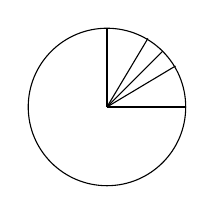
\begin{tikzpicture}
	\draw (0, 0) circle (1cm);
	\draw (0, 0) -- (1,0);
	\draw (0, 0) -- (0.87, 0.52);
	\draw (0, 0) -- (0.71, 0.71);
	\draw (0, 0) -- (0.52, 0.87);
	\draw (0, 0) -- (0, 1);
\end{tikzpicture}

To express every complex number $w^n = z$ we end up with the following generalization:
\begin{defn}[\textbf{Root of Unity}]
	\[\zeta^k = e^{\sfrac{2\pi ik}{n}}\]
\end{defn}
Which has the $n$th power given as:
\[ (\zeta^k)^n = ( e^{\sfrac{2\pi ik}{n}} )^n = e^{2\pi ik} = 1 \]
The points $w_k$ are just the product of $e^{\frac{i\theta}{n}}$ with all the $n$-th roots of unity:
\[w_k = e^{\sfrac{i\theta}{n}}\zeta^k\]

One of the \textbf{major results of the theory of complex variables} is to reduce the study of certain functions, including most of the 
common functions we know like exponentials, logarithms, sine, cosine; to power series, which can be approximated by polynomials.

Thus the power function is in some sense the unique basic function out of which the others are constructed.
